% Author and Copyright: Ruediger Gad
% This work is licensed under a Creative Commons Attribution-ShareAlike 3.0 Unported License.
% https://creativecommons.org/licenses/by-sa/3.0/
\documentclass[aspectratio=169]{beamer}
%[handout]
\usepackage[english]{babel}
\usepackage[utf8]{inputenc}
%\usepackage{avant}

\usepackage{listings}
\usepackage[T1]{fontenc}
\usepackage{textcomp}
\usepackage[variablett]{lmodern}
 
\lstset{
 basicstyle=\ttfamily,
 columns=fullflexible,
 upquote,
 keepspaces,
 escapeinside=||,
 literate={*}{{\char42}}1
 {-}{{\char45}}1
}

\usepackage{tabulary}
\usepackage{multirow}
\usepackage{dcolumn}
\newcolumntype{.}{D{.}{.}{-1}}
\usepackage{booktabs}
\usepackage{url}

\useoutertheme[footline=authorinstitutetitle,subsection=false]{miniframes}
\usetheme{Madrid}
%\usecolortheme[RGB={52,147,54}]{structure}
\usecolortheme{seagull}
\setbeamertemplate{navigation symbols}{}
%\setbeamertemplate{blocks}[rounded]

\setbeamercolor{footlinecolor}{fg=black,bg=white}
\setbeamertemplate{footline}{%
%  \pgfputat{\pgfxy(12,6.5)}{\pgfbox[center,base]{\includegraphics[width=1.6cm]{template_images/bert_kopf.png}}}
  \begin{beamercolorbox}[sep=0.5em,wd=\paperwidth]{footlinecolor}
  \begin{columns}
    \column{11cm}
      \tiny{\insertshortauthor}
      \vspace{0.05cm}
      \hrule
      \vspace{0.08cm}
      \tiny{\insertshorttitle}
    %\column{2cm}\hfill\includegraphics[width=2cm]{template_images/Logo_FHFFM}
    \column{4cm}\hfill %\includegraphics[width=1.5cm]{template_images/Logo_FHFFM_klein}
  \end{columns}
  \end{beamercolorbox}%
}


\title[Packet Capturing with the JVM and Clojure - Yes, we can!]{Packet Capturing with the JVM and Clojure\\Yes, we can!}
%\subtitle{Event-driven Network Analysis and Surveillance\\(ENeAS)}
\author[Ruediger Gad - Terma GmbH, Space - Darmstadt, Germany]{Ruediger Gad}
\institute[]{
  Terma GmbH, Space, Darmstadt, Germany
  }
\date{:clojureD\\2017-02-25}
%\logo{\includegraphics[width=3cm]{template_images/Logo_FHFFM.pdf}}


\begin{document}

	\begin{frame}[plain]
		\titlepage
	\end{frame}

  \begin{frame}
    \frametitle{Outline}

      \begin{itemize}
          \item Brief Introduction
          \item Packet Capturing \& the JVM
          \item Get up to speed.
          \item Domain Specific Language (DSL) for Data Transformation
          \item Adding Dynamic Capabilities
          \item Dynamic Self-adaptive Adjustments
      \end{itemize}
  \end{frame}

  \begin{frame}
    \frametitle{Computer Networks}

      \begin{center}
          \includegraphics[width=11cm]{images/self_adaptive_network_analysis_and_surveillance_system_8_without_NAaS}
      \end{center}
  \end{frame}

  \begin{frame}
    \frametitle{Network Monitoring}

      \begin{center}
          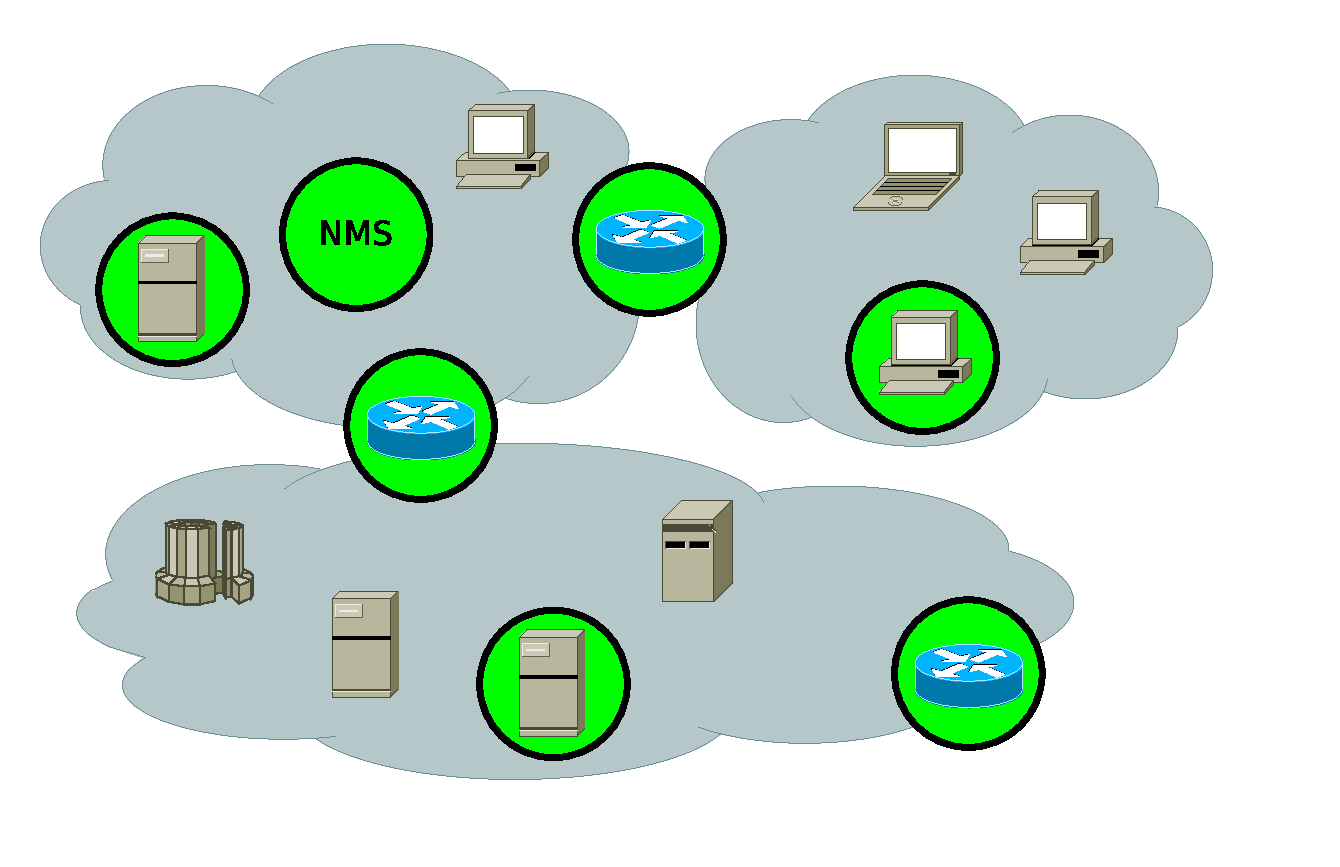
\includegraphics[width=11cm]{images/self_adaptive_network_analysis_and_surveillance_system_8}
      \end{center}
  \end{frame}

  \begin{frame}
    \frametitle{Network Monitoring Use Case Overview}

      \begin{itemize}
          \item Requirements
              \begin{itemize}
                  \item Distribution, Flexibility, Data Analysis, \ldots{}
              \end{itemize}
          \item JVM-based
               \begin{itemize}
                   \item Re-use Existing Libraries\\
                         Communication Middleware, Data Processing, \ldots{}
               \end{itemize}
           \item Clojure
               \begin{itemize}
                   \item Powerful, Dynamic, \ldots{}
               \end{itemize}
          \item Packet Capturing as ``Worst Case Scenario''
              \begin{itemize}
                  \item Data Throughput
                  \item Data Volume
%                  \item Byte Arrays to Java Types
              \end{itemize}
      \end{itemize}
  \end{frame}

%  \begin{frame}
%      \frametitle{Use Case \& Requirements Evolved}
%
%      \begin{itemize}
%          \item Maintainability
%          \item Extendibility
%          \item Performance
%          \item Flexibility
%          \item Dynamic Adjustments
%          \item Output Formats
%          \item Meta Data
%          \item Pre-processing
%          \item \ldots{}
%      \end{itemize}
%  \end{frame}

  \begin{frame}
      \frametitle{Packet Capturing (Pcap) \& the JVM}

      \begin{center}
          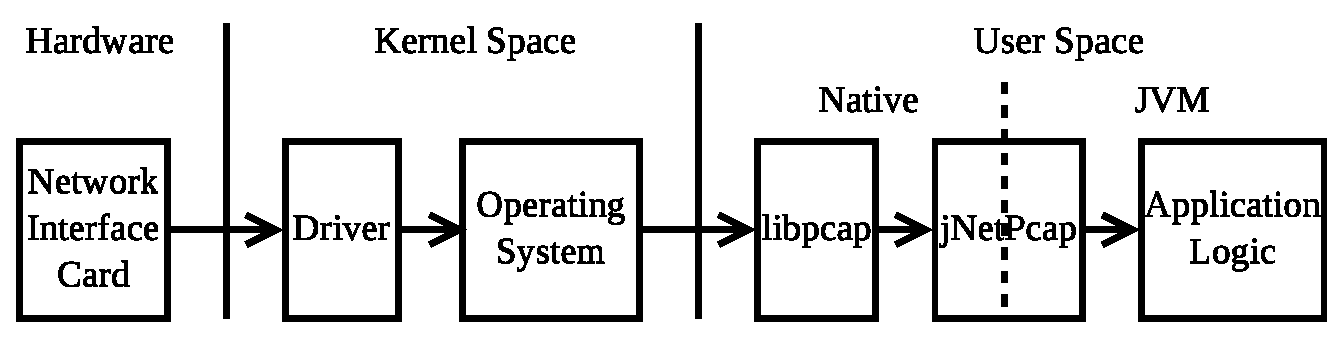
\includegraphics[width=15cm]{images/packet_capturing_data_flow}
      \end{center}
  \end{frame}

  \begin{frame}
      \frametitle{Pcap \& the JVM, Per Packet Forwarding}

      \begin{center}
          \includegraphics[width=15cm]{images/jnetpcap_byte_buffer}
      \end{center}
  \end{frame}

  \begin{frame}
      \frametitle{Pcap \& the JVM, Packet Bulk Forwarding}

      \begin{center}
          \includegraphics[width=15cm]{images/modified_jnetpcap_bulk_processing_direct_buffer}
      \end{center}
  \end{frame}

  \begin{frame}
      \frametitle{Pcap \& the JVM, Improved Packet Bulk Forwarding}

      \begin{center}
          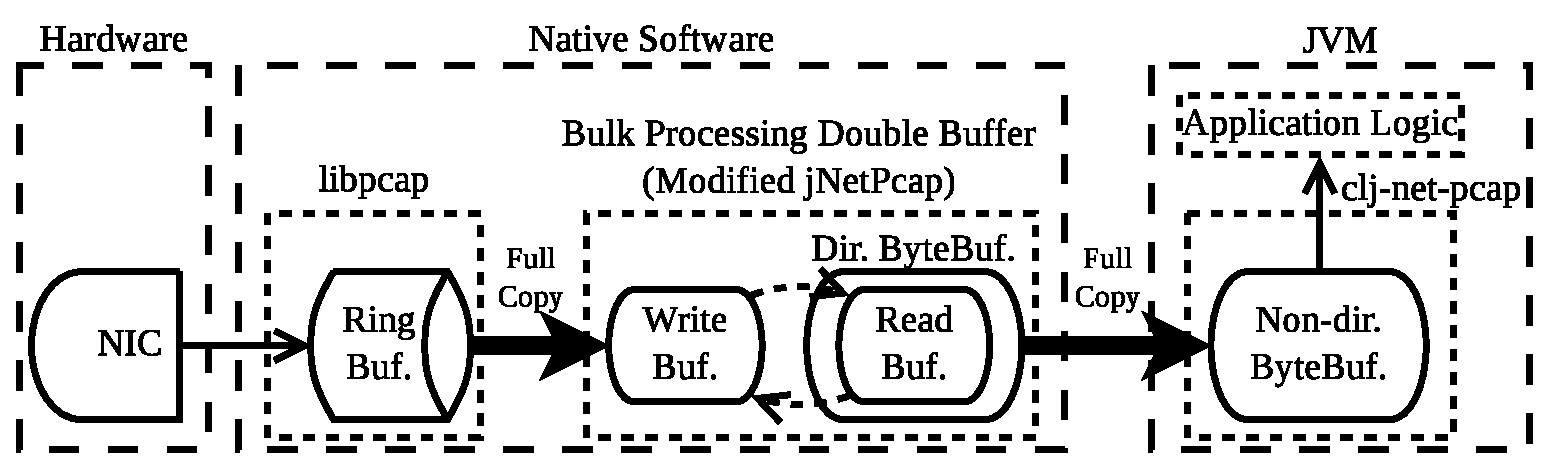
\includegraphics[width=15cm]{images/modified_jnetpcap_bulk_processing_double_buffer}
      \end{center}
  \end{frame}

  \begin{frame}
      \frametitle{Raw Pcap Performance Comparison}

      \begin{center}
          \includegraphics[width=15cm]{images/comparison}
      \end{center}
  \end{frame}



  \begin{frame}
    \frametitle{Making Sense of Raw Packet Data}
    \begin{itemize}
        \item Raw Packet Data (Byte Arrays) to Java Types
        \item ``Address Fields'' (Offsets)
        \item Name Data
        \item Transform Data
            \begin{itemize}
                \item Integer Values (4, 8, 16, 32 bit)
                \item Timestamps
                \item Addresses (IP, MAC)
            \end{itemize}
        \item Output Data Type
    \end{itemize}
  \end{frame}



\begin{frame}[fragile]
\frametitle{Data Extraction DSL}
\begin{lstlisting}[caption=Extraction DSL Expression Example]
{:type :java-map
 :rules [[ts (timestamp 0)]
         [len (int32 12)]
         [ipDst (ipv4-address ipv4-dst)]
         [udpDst (int16 udp-dst)]]}
\end{lstlisting}
\begin{lstlisting}[caption=Extraction Function based on DSL]
(fn [ba]
  (doto (java.util.HashMap.)
    (.put "ts" (timestamp ba 0))
    (.put "len" (int32 ba 12))
    (.put "ipDst" (ipv4-address ba 46))
    (.put "udpDst" (int16 ba 52))))
\end{lstlisting}
\end{frame}


\begin{frame}
\frametitle{Data Extraction Throughput Comparison}
\begin{table}
%    \caption{Throughput Comparison}
\centering
\begin{tabular}[!htb]{l r r}
    Method       & Throughput [$\bar{x}$] & [$sd(x)$] \\\toprule
%    Old Extr. (Map) Full     &   265789      &   401 \\
    jNetPcap        &   265.7 kpps &  10.4 kpps     \\
    DSL             &   612.2 kpps &   8.8 kpps     \\
%    Hard-coded      &   657.1 kpps &  18.5 kpps     \\
%    Old Extr. (Bean) Full    &   273443      &   401 \\
%    jNetPcap (Bean)           &   274.9 kpps ; 21.9 kpps      &   396 \% \\
%    Byte Array (Map)          &   657.1 kpps ; 18.5 kpps      &   201 \% \\
%    Byte Array (Bean)         &   772.6 kpps ; 37.3 kpps      &   200 \% \\\bottomrule
\end{tabular}
\label{tbl:extraction_performance_comparison}
\end{table}
\end{frame}

  \begin{frame}
    \frametitle{What if throughput demands increase further?}
      \begin{columns}
          \column{9cm}
    \begin{itemize}
        \item<2-> Do nothing?\\
              $\rightarrow$ Random Drops of ``Rows''
        \item<3-> Apply sampling?\\
              $\rightarrow$ More ``Controlled'' Drops of Rows
        \item<4-> Reduce extraction operations / extracted fields?\\
              $\rightarrow$ ``Drop columns'' in favor of rows.\\
        \item<5-> $\rightarrow$ Adjust DSL expression rules.
    \end{itemize}
          \column{5cm}
        \includegraphics<1>[width=4.5cm]{images/columns_and_rows}
        \includegraphics<2>[width=4.5cm]{images/columns_and_rows_random_row_drops}
        \includegraphics<3>[width=4.5cm]{images/columns_and_rows_controlled_row_drops}
        \includegraphics<4->[width=4.5cm]{images/columns_and_rows_controlled_column_drops}
      \end{columns}
  \end{frame}


\begin{frame}
\frametitle{Throughput for Varying DSL Expression Complexity}
\begin{table}
%    \caption{Throughput for Varying DSL Expression Complexity}
\centering
\begin{tabular}[!htb]{l r r}
    Method       &  Capture Rate [$\bar{x}$] & [$sd(x)$]    \\\toprule
    DSL 1        &   612.2 kpps &   8.8 kpps \\
    DSL 2        &   726.4 kpps &   9.1 kpps \\
    DSL 3        &  1114.8 kpps &  46.4 kpps \\
    DSL 4        &  1478.7 kpps & 146.9 kpps \\\bottomrule
\end{tabular}
\label{tbl:dsl_performance_comparison}
\end{table}
\pause
    \begin{itemize}
        \item Do this dynamically.
        \item At Run-time
    \end{itemize}
\end{frame}



\begin{frame}[fragile]
\frametitle{Defining a Clojure Function at Run-time}
%\begin{lstlisting}[caption=Clojure REPL Example for Defining a Function at Run-time from a User Input String]
\begin{lstlisting}[]
=> (def f1-str "(clojure.core/fn [] (clojure.core/println \"foo\"))")
#'user/f1-str|\pause|
=> (def f1-list (binding [*read-eval* false] (read-string f1-str)))
#'user/f1-list|\pause|
=> (type f1-list)
clojure.lang.PersistentList|\pause|
=> f1-list
(clojure.core/fn [] (clojure.core/println "foo"))|\pause|
=> (def f1 (eval f1-list))
#'user/f1|\pause|
=> (f1)
foo
nil
\end{lstlisting}
\end{frame}


%\begin{frame}[fragile]
%\frametitle{Defining a Function with Arguments at Run-time}
%\begin{lstlisting}[caption=Clojure REPL Example for Defining a Function with Arguments at Run-time,basicstyle=\normalsize]
%=> (def x 'x-sym)
%#'user/x
%=> (def f2-list `(fn [~x] (inc ~x)))
%#'user/f2-list
%=> f2-list
%(clojure.core/fn [x-sym] (clojure.core/inc x-sym))
%=> (def f2 (eval f2-list))
%#'user/f2
%=> (f2 41)
%42
%\end{lstlisting}
%\end{frame}


\begin{frame}[fragile]
\frametitle{Function in Atom for Dynamic Behaviour}
%\begin{lstlisting}[caption=Function in Atom for Dynamic Behaviour]
\begin{lstlisting}[]
=> (def f-atom (atom (fn [x] (inc x))))
#'user/f-atom|\pause|
=> (@f-atom 41)                        
42|\pause|
=> (reset! f-atom (fn [x] (dec x)))
#object[user$eval16$fn__17 0x45ac5f9b ...|\pause|
=> (@f-atom 41)                    
40
\end{lstlisting}
\end{frame}



\begin{frame}[fragile]
\frametitle{Improving Dynamic Behaviour via Watch}
\begin{lstlisting}[caption=Improving Dynamic Behaviour via Watch]
...
=> (def f (atom (eval @f-list)))                            
#'user/f|\pause|
=> (@f 41)                                
42|\pause|
=> (add-watch f-list :id (fn [k r o n-val] (reset! f (eval n-val))))
#object[clojure.lang.Atom 0xc7045b9 ...|\pause|
=> (reset! f-list `(fn [~x] (dec ~x)))                      
(clojure.core/fn [x-sym] (clojure.core/dec x-sym))|\pause|
=> (@f 41)                                                  
40
\end{lstlisting}
\end{frame}



  \begin{frame}
    \frametitle{Where to go from here?}
    \begin{itemize}
        \item Dynamic Adjustments\\
              $\rightarrow$ Work.
        \item Manual Adjustments?
            \begin{itemize}
                \item Slow, Labour Intensive, Impossible(?!), \ldots{}
            \end{itemize}
        \item Automatic Dynamic Adjustments\\
              $\rightarrow$ Self-adaptive Adjustments
    \end{itemize}
  \end{frame}



\begin{frame}
    \frametitle{Self-adaptivity Feedback Loop (``MAPE-K'')}
    \begin{center}
        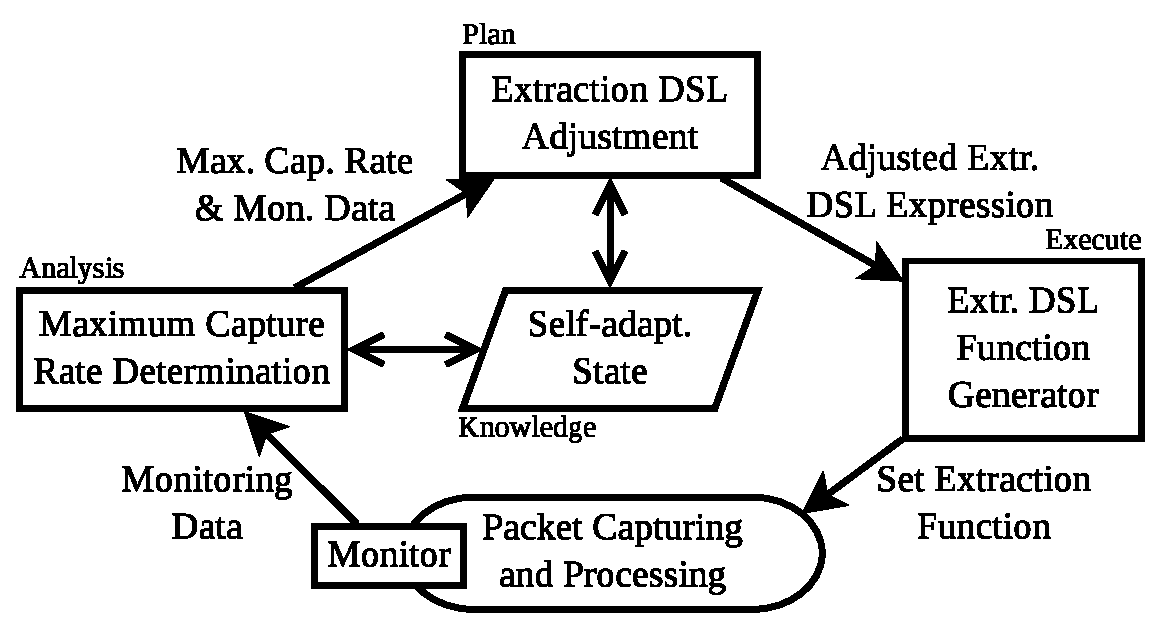
\includegraphics[width=11cm]{images/control_loop_overview}
    \end{center}
\end{frame}



\begin{frame}
    \frametitle{Self-adaptive Performance Adjustments}
    \begin{center}
        \includegraphics[width=\linewidth]{images/sa_test_66}
    \end{center}
\end{frame}





  \begin{frame}
      \frametitle{Summary}

    \begin{itemize}
        \item Introduction
            \begin{itemize}
                \item Computer Networks \& Computer Network Monitoring
            \end{itemize}
        \item Packet Capturing with the JVM
            \begin{itemize}
                \item Hardware $\rightarrow$ Kernel Space $\rightarrow$ User Space $\rightarrow$ JVM
                \item Per Packet vs. Bulk Data Forwarding
                \item Different Memory Management Approaches
                \item Improvement by about x5.6 (up to approximately 10 Gbps)
            \end{itemize}
        \item Data Processing DSL
            \begin{itemize}
                \item Dynamic Data Extraction
            \end{itemize}
        \item Self-adaptive Performance-based Data Processing Adjustments
    \end{itemize}
  \end{frame}

  \begin{frame}
      \frametitle{Summary continued}

    \begin{itemize}
%        \item Performance Improvements (More Possible?)
        \item DSL Abstraction Benefits
            \begin{itemize}
                \item Extendibility, Maintainability, Flexibility, \ldots{}
            \end{itemize}
        \item Clojure-related Aspects
            \begin{itemize}
                \item Homoiconic, Dynamic Capabilities, JVM-based, \ldots{}
            \end{itemize}
        \item Implementations: Open Source Software\\
              \url{https://github.com/ruedigergad/clj-net-pcap}\\
              \url{https://github.com/ruedigergad/dsbdp}
    \end{itemize}
      \pause
    \begin{block}{Packet Capturing with the JVM and Clojure?}
      \begin{center} Yes, we can! \end{center}
    \end{block}
  \end{frame}

  \begin{frame}[c]
    \frametitle{End}
    \begin{block}{Thank you very much for your attention!}
      \begin{center} Questions? \end{center}
    \end{block}
    \vspace{0.5cm}
    \begin{center}Ruediger Gad\\Terma GmbH, Space\\Darmstadt, Germany\end{center}
        \begin{center}ruga@terma.com\\r.c.g@gmx.de\\\url{https://github.com/ruedigergad}\\\url{https://ruedigergad.com}\end{center}
  \end{frame}
\end{document}

